% ------------------------------------------------------------------
\documentclass[12 pt]{article} % A4 paper set by geometry package below
\pagenumbering{arabic}
\setlength{\parindent}{10 mm}
\setlength{\parskip}{12 pt}

% Nimbus Sans font should be reasonably legible
\usepackage{helvet}
\renewcommand{\familydefault}{\sfdefault}
\usepackage[T1]{fontenc}  % Without this \textsterling produces $

% Section header spacing
\usepackage{titlesec}
\titlespacing\section{0pt}{12pt plus 4pt minus 2pt}{0pt plus 2pt minus 2pt}
\titlespacing\subsection{0pt}{12pt plus 4pt minus 2pt}{0pt plus 2pt minus 2pt}
\titlespacing\subsubsection{0pt}{12pt plus 4pt minus 2pt}{0pt plus 2pt minus 2pt}

\usepackage{amsmath}
\usepackage{amssymb}
\usepackage{graphicx}
\usepackage{verbatim}    % For comment
\usepackage[paper=a4paper, marginparwidth=0 cm, marginparsep=0 cm, margin=2.5 cm, includemp]{geometry}
\usepackage[pdftex, pdfstartview={FitH}, pdfnewwindow=true, colorlinks=true, citecolor=blue, filecolor=blue, linkcolor=blue, urlcolor=blue, pdfpagemode=UseNone]{hyperref}

% Put module code and last-modified date in footer
\usepackage{fancyhdr}
\pagestyle{fancy}
\fancyhf{}
\renewcommand{\headrulewidth}{0pt}
\cfoot{{\small \thisunit}\hfill \thepage\hfill {\small \moddate}}

% Hopefully address Canvas complaints about pdf tagging
%\usepackage[tagged]{accessibility}
\hypersetup {
  pdfauthor={David Schaich},
  pdftitle={StatMech Tutorial},
}
% ------------------------------------------------------------------



% ------------------------------------------------------------------
% Shortcuts
\newcommand{\De}{\ensuremath{\Delta} }
\newcommand{\la}{\ensuremath{\lambda} }
\newcommand{\lath}{\ensuremath{\la_{\mathrm{th}}} }
\newcommand{\Om}{\ensuremath{\Omega} }
% ------------------------------------------------------------------



% ------------------------------------------------------------------
\begin{document}
\newcommand{\thisunit}{MATH327 Tutorial (Mixing)}
\newcommand{\moddate}{Last modified 5 Mar.~2025}
\begin{center}
  {\Large \textbf{MATH327: StatMech and Thermo, Spring 2025}} \\[12 pt]
  {\Large \textbf{Tutorial exercises \ --- \ Mixing entropy}} \\[24 pt]
\end{center}

These exercises will be introduced in our 6 March tutorial, and you'll have the week until our next tutorial on 13 March to work on them.
They delve deeper into the particle mixing thought experiment we used to introduce the mixing entropy earlier this week, in which we obtain three systems $\{\Om_0, \Om_C, \Om_F\}$ by removing and re-inserting a wall.
We want to ensure that the entropy obeys the second law, $S_0 \leq S_C \leq S_F$.

To simplify things, consider the special case illustrated by the figure below.
Here \textit{all} $2N$ particles have indistinguishable physical properties, \textit{except} that those initially in the left compartment (the ``reds'') are distinguishable from those in right compartment (the ``blues'') by their colour.
After mixing and re-separation, red and blue particles can appear on either side of the wall in the final system $\Om_F$.

\begin{center}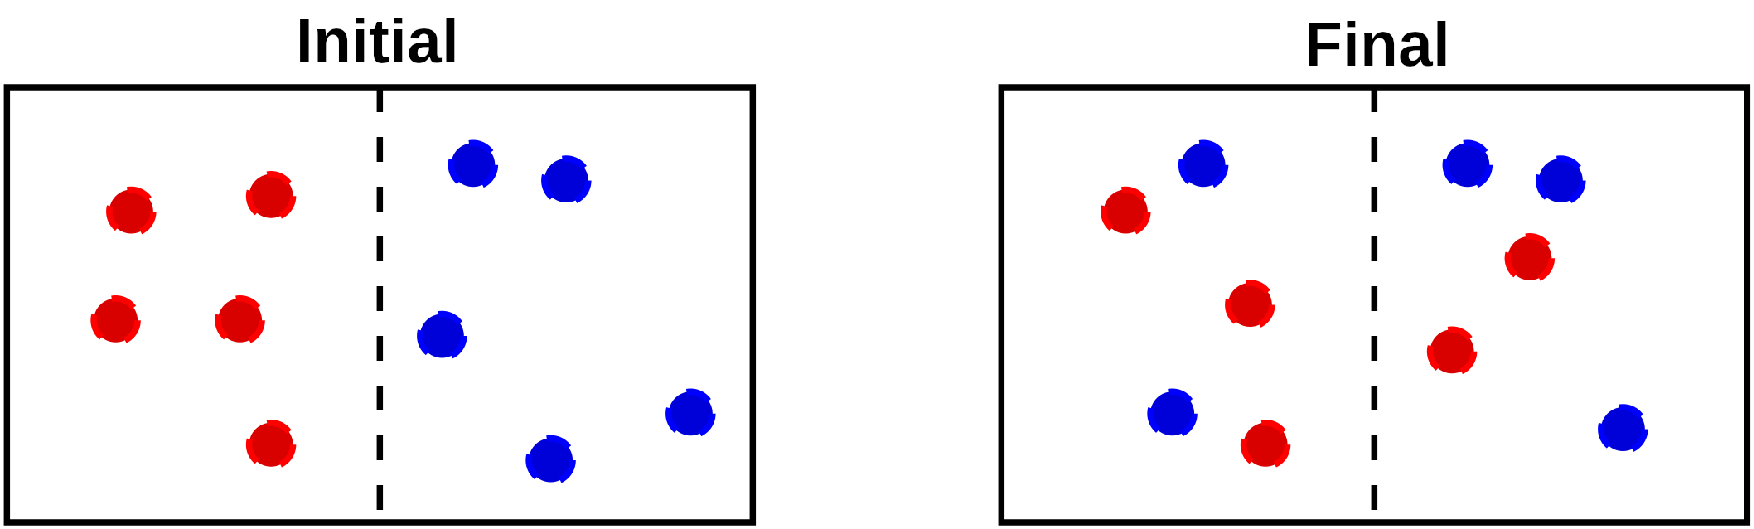
\includegraphics[width=0.8\textwidth]{figs/mix.pdf}\end{center}

\textbf{The first task} is to check $S_0 \leq S_C$, or equivalently $\De S_{\text{mix}} \geq 0$.
Since the combined system $\Om_C$ has two (distinguishable) sets of $N$ (indistinguishable) particles in volume $2V$, its partition function is
\begin{equation*}
  Z_C = \frac{1}{N!} \frac{1}{N!} Z_1^{2N} = \frac{1}{N!} \frac{1}{N!} \left(\frac{2V}{\lath^3}\right)^{2N} \qquad \mbox{with} \qquad \lath = \sqrt{\frac{2\pi\hbar^2}{mT}},
\end{equation*}
where $Z_1 = 2V / \lath^3$ is the single-particle partition function.
It may be useful to use properties of logarithms to translate entropy differences to partition function ratios.

\textbf{The second task} is to check $S_C \leq S_F$ by computing the final entropy $S_F$.
First, compute the partition function $Z_F$ of the two re-separated systems, by summing over all ways of dividing the red and blue particles between them.
We can continue to use the Gibbs approximation that both systems end up with $N \gg 1$ particles.
This special case of the \href{https://en.wikipedia.org/wiki/Zhu_Shijie}{Zhu}--\href{https://en.wikipedia.org/wiki/Alexandre-Theophile_Vandermonde}{Vandermonde} \href{https://en.wikipedia.org/wiki/Vandermonde's_identity}{identity} for the \href{https://mathworld.wolfram.com/BinomialSums.html}{binomial sum} may be useful:
\begin{equation*}
  \sum_{k = 0}^N \binom{N}{k}^2 = \binom{2N}{N}.
\end{equation*}
Finally, use $Z_F$ to determine $S_F$.
If you apply Stirling's formula, you may find it interesting to repeat your work with and without the $\log\left(\sqrt{2\pi N}\right)$ terms.

\end{document}
% ------------------------------------------------------------------
